\documentclass[]{article}
\usepackage{lmodern}
\usepackage{amssymb,amsmath}
\usepackage{ifxetex,ifluatex}
\usepackage{fixltx2e} % provides \textsubscript
\ifnum 0\ifxetex 1\fi\ifluatex 1\fi=0 % if pdftex
  \usepackage[T1]{fontenc}
  \usepackage[utf8]{inputenc}
\else % if luatex or xelatex
  \ifxetex
    \usepackage{mathspec}
  \else
    \usepackage{fontspec}
  \fi
  \defaultfontfeatures{Ligatures=TeX,Scale=MatchLowercase}
\fi
% use upquote if available, for straight quotes in verbatim environments
\IfFileExists{upquote.sty}{\usepackage{upquote}}{}
% use microtype if available
\IfFileExists{microtype.sty}{%
\usepackage{microtype}
\UseMicrotypeSet[protrusion]{basicmath} % disable protrusion for tt fonts
}{}
\usepackage[margin=1in]{geometry}
\usepackage{hyperref}
\hypersetup{unicode=true,
            pdftitle={Fundamentals of Computing and Data Display - Term Paper},
            pdfauthor={Xuefei Li \& Tianheao Wang},
            pdfborder={0 0 0},
            breaklinks=true}
\urlstyle{same}  % don't use monospace font for urls
\usepackage{color}
\usepackage{fancyvrb}
\newcommand{\VerbBar}{|}
\newcommand{\VERB}{\Verb[commandchars=\\\{\}]}
\DefineVerbatimEnvironment{Highlighting}{Verbatim}{commandchars=\\\{\}}
% Add ',fontsize=\small' for more characters per line
\usepackage{framed}
\definecolor{shadecolor}{RGB}{248,248,248}
\newenvironment{Shaded}{\begin{snugshade}}{\end{snugshade}}
\newcommand{\AlertTok}[1]{\textcolor[rgb]{0.94,0.16,0.16}{#1}}
\newcommand{\AnnotationTok}[1]{\textcolor[rgb]{0.56,0.35,0.01}{\textbf{\textit{#1}}}}
\newcommand{\AttributeTok}[1]{\textcolor[rgb]{0.77,0.63,0.00}{#1}}
\newcommand{\BaseNTok}[1]{\textcolor[rgb]{0.00,0.00,0.81}{#1}}
\newcommand{\BuiltInTok}[1]{#1}
\newcommand{\CharTok}[1]{\textcolor[rgb]{0.31,0.60,0.02}{#1}}
\newcommand{\CommentTok}[1]{\textcolor[rgb]{0.56,0.35,0.01}{\textit{#1}}}
\newcommand{\CommentVarTok}[1]{\textcolor[rgb]{0.56,0.35,0.01}{\textbf{\textit{#1}}}}
\newcommand{\ConstantTok}[1]{\textcolor[rgb]{0.00,0.00,0.00}{#1}}
\newcommand{\ControlFlowTok}[1]{\textcolor[rgb]{0.13,0.29,0.53}{\textbf{#1}}}
\newcommand{\DataTypeTok}[1]{\textcolor[rgb]{0.13,0.29,0.53}{#1}}
\newcommand{\DecValTok}[1]{\textcolor[rgb]{0.00,0.00,0.81}{#1}}
\newcommand{\DocumentationTok}[1]{\textcolor[rgb]{0.56,0.35,0.01}{\textbf{\textit{#1}}}}
\newcommand{\ErrorTok}[1]{\textcolor[rgb]{0.64,0.00,0.00}{\textbf{#1}}}
\newcommand{\ExtensionTok}[1]{#1}
\newcommand{\FloatTok}[1]{\textcolor[rgb]{0.00,0.00,0.81}{#1}}
\newcommand{\FunctionTok}[1]{\textcolor[rgb]{0.00,0.00,0.00}{#1}}
\newcommand{\ImportTok}[1]{#1}
\newcommand{\InformationTok}[1]{\textcolor[rgb]{0.56,0.35,0.01}{\textbf{\textit{#1}}}}
\newcommand{\KeywordTok}[1]{\textcolor[rgb]{0.13,0.29,0.53}{\textbf{#1}}}
\newcommand{\NormalTok}[1]{#1}
\newcommand{\OperatorTok}[1]{\textcolor[rgb]{0.81,0.36,0.00}{\textbf{#1}}}
\newcommand{\OtherTok}[1]{\textcolor[rgb]{0.56,0.35,0.01}{#1}}
\newcommand{\PreprocessorTok}[1]{\textcolor[rgb]{0.56,0.35,0.01}{\textit{#1}}}
\newcommand{\RegionMarkerTok}[1]{#1}
\newcommand{\SpecialCharTok}[1]{\textcolor[rgb]{0.00,0.00,0.00}{#1}}
\newcommand{\SpecialStringTok}[1]{\textcolor[rgb]{0.31,0.60,0.02}{#1}}
\newcommand{\StringTok}[1]{\textcolor[rgb]{0.31,0.60,0.02}{#1}}
\newcommand{\VariableTok}[1]{\textcolor[rgb]{0.00,0.00,0.00}{#1}}
\newcommand{\VerbatimStringTok}[1]{\textcolor[rgb]{0.31,0.60,0.02}{#1}}
\newcommand{\WarningTok}[1]{\textcolor[rgb]{0.56,0.35,0.01}{\textbf{\textit{#1}}}}
\usepackage{longtable,booktabs}
\usepackage{graphicx,grffile}
\makeatletter
\def\maxwidth{\ifdim\Gin@nat@width>\linewidth\linewidth\else\Gin@nat@width\fi}
\def\maxheight{\ifdim\Gin@nat@height>\textheight\textheight\else\Gin@nat@height\fi}
\makeatother
% Scale images if necessary, so that they will not overflow the page
% margins by default, and it is still possible to overwrite the defaults
% using explicit options in \includegraphics[width, height, ...]{}
\setkeys{Gin}{width=\maxwidth,height=\maxheight,keepaspectratio}
\IfFileExists{parskip.sty}{%
\usepackage{parskip}
}{% else
\setlength{\parindent}{0pt}
\setlength{\parskip}{6pt plus 2pt minus 1pt}
}
\setlength{\emergencystretch}{3em}  % prevent overfull lines
\providecommand{\tightlist}{%
  \setlength{\itemsep}{0pt}\setlength{\parskip}{0pt}}
\setcounter{secnumdepth}{0}
% Redefines (sub)paragraphs to behave more like sections
\ifx\paragraph\undefined\else
\let\oldparagraph\paragraph
\renewcommand{\paragraph}[1]{\oldparagraph{#1}\mbox{}}
\fi
\ifx\subparagraph\undefined\else
\let\oldsubparagraph\subparagraph
\renewcommand{\subparagraph}[1]{\oldsubparagraph{#1}\mbox{}}
\fi

%%% Use protect on footnotes to avoid problems with footnotes in titles
\let\rmarkdownfootnote\footnote%
\def\footnote{\protect\rmarkdownfootnote}

%%% Change title format to be more compact
\usepackage{titling}

% Create subtitle command for use in maketitle
\providecommand{\subtitle}[1]{
  \posttitle{
    \begin{center}\large#1\end{center}
    }
}

\setlength{\droptitle}{-2em}

  \title{Fundamentals of Computing and Data Display - Term Paper}
    \pretitle{\vspace{\droptitle}\centering\huge}
  \posttitle{\par}
  \subtitle{Understanding the ``Depression'' from Twitter activity:an exploratory
study}
  \author{Xuefei Li \& Tianheao Wang}
    \preauthor{\centering\large\emph}
  \postauthor{\par}
      \predate{\centering\large\emph}
  \postdate{\par}
    \date{2019-12-13}


\begin{document}
\maketitle

{
\setcounter{tocdepth}{2}
\tableofcontents
}
\hypertarget{abstract}{%
\subsection{Abstract}\label{abstract}}

xxx

\hypertarget{introduction}{%
\subsection{Introduction}\label{introduction}}

\hypertarget{research-background}{%
\subsubsection{Research background}\label{research-background}}

Depressive disorders have become an increasingly serious and public
mental health issue around the world. Among all the public health
problems, the depression is more easily leading to suicide globally,
which constitutes a huge challenge for public health. However, relevant
research is mainly conducted with experimental psychological data,
large-scale available quantifiable preliminary data is insufficient for
study. To obtain preliminary data, social media is a perfect fit for
studying mental health in both individual and overall trends in the
population, because people are increasingly likely to post feelings and
thoughts with the others, expressing DEPRESSED EMOTION on social media
meanwhile, while their expressive behavior is different to each other.
Thus, language use, social expression and their interaction are
uncovering indicators of mental health. Recently, there appears to be
numerous studies using social media, especially twitter data to
investigate people's emotions and political opinions, as well as
predicting the future trends.

\hypertarget{literature-review}{%
\subsubsection{Literature review}\label{literature-review}}

Depression has become a major public health problem around the world.
According to the World Health Organization (WHO), depression is a common
mental disorder. Globally, more than 264 million people of all ages
suffer from depression (Centers for Disease Control and Prevention (CDC)
2012). Depression is a leading cause of disability worldwide and is a
major contributor to the overall global burden of disease, which is
believed to be responsible for the more than 30,000 suicides each year
(Luoma, Martin, and Pearson 2002). It involves repeated depressive
period, during which person will experience depressed mood, loss of
interest and enjoyment, and reduced energy leading to diminished
activity. However, there is a problem of insufficient diagnosis and
treatment for depression. It can be hard to accurately diagnose
depression because it can look so different from person to person
(Smith, Renshaw, and Bilello 2013). More important, several researches
have found that a good portion of people with mental disorder is not
getting help. Olfson, Blanco and Marcus (2016) screened more than 46000
adults for depression and found that 8.4\% have a positive test results
for depression. However, only less than 30\% of the study participants
with depression actually sought treatment.

According to a survey from the High Watch Recovery Center, there are
several reasons for people who need help for a mental health issue but
don't seek it. First, people may be afraid of being stigmatized. Second,
people may not realize that they do need assistances from professionals.
Furthermore, people's circumstances and some practical issues may
prevent them from seeking help. For example, economic level, geographic
location, availability of psychologists, etc. Also, there is a
probability that people just are scared of the treatment or therapy,
misleading by disturbing conceptions such as the old-fashioned
lobotomies or electroconvulsive therapy. In general, depression as a
serious mental health issue has become prevalent in recent years while
lack of efficient methods to detect depression.

In the context of all the challenges, social media has become a
potential source to detect people's behavior and mental process. People
are increasingly using social media platforms like Twitter, Facebook and
Instagram to express their thoughts and share their opinions with
contacts. Peoples' tweets can be considered as their true emotions and
feelings in naturalistic settings, recording their real-time daily
activities and happenings (Choudhury et al. 2013). On contrary to
traditional subjective self-reporting measures, large-scale and
fine-grained records of users' activities in social media allow
researchers using objective information to recognize depression (Tsugawa
et al. 2015).

Although there might be social desirability in the circumstance since
social media is a public platform that everyone can see the contents.
However, we can still consider social media as a reliable method for
capturing the thoughts, mood, communication and socialization of
individuals. The languages in social media postings may indicate
feelings of worthlessness, guilt, helplessness, and self-hatred that
characterize depression as manifested in our daily life (Choudhury,
Counts, and Horvitz 2013). Additionally, the etiology of depression
typically includes social environmental factors (Rosenquist, Fowler, and
Christakis 2002). Capturing the depression sufferers' social context in
a manner that might help detect depression in populations. Park et al.
(2012) provided initial evidence that twitter users do expose their
depression and even their therapy and treatment of depression in tweets
(Park, Cha, and Cha 2012). It is also possible that identifying
depression by analyzing textual data from sentences written by the
individuals (Resnik, Garron, and Resnik 2013). Meanwhile, researchers
evaluated the effectiveness of using social media activities data to
estimate the degree of depression and found that features obtained from
user activities can be used to predict depression with an accuracy of
69\% (Tsugawa et al. 2015). All those works highlighted the potential of
social media, especially Twitter as an effective source of signals to
analyze or even predict current or future episodes of depression.

However, there is few previous researches use large-scale Twitter data,
only focusing on small samples. Meanwhile, previous research did not
analyze the attributes of depressed individual, especially their
activities on Twitter. Most importantly, previous studies did not group
participants entering the research to control the features obtained from
on-line activities of the participants, so it was unable to compare and
obtain causality between groups. Thus, in this paper:

\begin{itemize}
\item
  We conducted a quasi-experiemnt, which can also be stated as
  field-test, divided the participants into three groups and
  investigated their differences in activities on the Twitter platform.
\item
  Furthermore, we analyzed the texts of different groups of
  participants, exploring the content as well as sentiments of the
  individuals.
\item
  Finally, we tried to investigate some relationships between features
  of Twitter users and their sentimental performances.
\end{itemize}

\hypertarget{method}{%
\subsection{Method}\label{method}}

\hypertarget{data-sources}{%
\subsubsection{Data sources}\label{data-sources}}

In this study, we collected data directly from Twitter. All data we
obtain is public, posted between December 1st to December 8th in 2019,
and made available from Twitter via their application programming
interface (API). Specifically, it does not include any data that
language is not English. All the tweets we collected are original posts,
in other words, are not retweets. Tweets texts that contain hashtags and
uniform resource locator are also excluded from our data.

\begin{Shaded}
\begin{Highlighting}[]
\KeywordTok{create_token}\NormalTok{(}
  \DataTypeTok{app =} \StringTok{"Data Display Social Research"}\NormalTok{,}
  \DataTypeTok{consumer_key =} \StringTok{"kSGIiodRghgYq289SZBRP5hlO"}\NormalTok{,}
  \DataTypeTok{consumer_secret =} \StringTok{"jFLbGoOsgxuhon4YLX51Lb5Q79EgIwjjJSVYu3SZEa6x7EkLl2"}\NormalTok{,}
  \DataTypeTok{access_token =} \StringTok{"1181245045287948288-tjS90xmIaMmRsAAEaCDUuM8jkhlbE9"}\NormalTok{,}
  \DataTypeTok{access_secret =} \StringTok{"4K45yuHd4gSXZXMeRu11Tp8SsYda7NXzzYKSC41XjDw12"}
\NormalTok{)}

\KeywordTok{create_token}\NormalTok{(}
  \DataTypeTok{app =} \StringTok{"Data Display Social Research"}\NormalTok{,}
  \DataTypeTok{consumer_key =} \StringTok{"3RdnGQ0hETW7LHbQdZtI14VRD"}\NormalTok{,}
  \DataTypeTok{consumer_secret =} \StringTok{"0mxU7gGQSgSF2NgYJVuCC9au026ut5ncUJLr13ppU8Unw9a2Qx"}\NormalTok{,}
  \DataTypeTok{access_token =} \StringTok{"1181245045287948288-WkVfbTxp82YMBP64F5GjH6oyt9Ux8d"}\NormalTok{,}
  \DataTypeTok{access_secret =} \StringTok{"gWOYYYVyv7BzUhYSy8p4a3HXw5MPGi8RxUi30qciaQdEf"}
\NormalTok{)}

\KeywordTok{get_token}\NormalTok{()}
\end{Highlighting}
\end{Shaded}

\hypertarget{data-collection}{%
\subsubsection{Data collection}\label{data-collection}}

We collected three groups of data separately. The first group is general
``Depression Group'', which is the individuals whose tweets text
contained the word ``depression''. We first search the latest 18k
English tweets including the keyword ``depression'' several times in
one-week window, combine them into a dataset and delete observations
that duplicated in every column. Then we set a random sampling to select
20k observations as group 1.

\begin{Shaded}
\begin{Highlighting}[]
\NormalTok{dp1 <-}\StringTok{ }\KeywordTok{search_tweets}\NormalTok{(}\StringTok{"depression"}\NormalTok{, }\DataTypeTok{lang =} \StringTok{"en"}\NormalTok{, }\DataTypeTok{include_rts =} \OtherTok{FALSE}\NormalTok{, }\DataTypeTok{n =} \DecValTok{18000}\NormalTok{)}
\NormalTok{dp1 <-}\StringTok{ }\KeywordTok{subset}\NormalTok{(dp1, }\KeywordTok{is.na}\NormalTok{(dp1}\OperatorTok{$}\NormalTok{hashtags))}
\NormalTok{dp1 <-}\StringTok{ }\KeywordTok{subset}\NormalTok{(dp1, }\KeywordTok{is.na}\NormalTok{(dp1}\OperatorTok{$}\NormalTok{url))}
\NormalTok{dp1 <-}\StringTok{ }\NormalTok{dp1 }\OperatorTok
\StringTok{  }\KeywordTok{select}\NormalTok{ (user_id, created_at, text, source, display_text_width, location, }
\NormalTok{          followers_count, friends_count, listed_count, statuses_count, }
\NormalTok{          favourites_count, account_created_at)}
\NormalTok{dp1 <-}\StringTok{ }\KeywordTok{as.data.frame}\NormalTok{(dp1)}
\KeywordTok{save_as_csv}\NormalTok{(dp1, }\StringTok{"dp1-Date-Time.csv"}\NormalTok{)}
\end{Highlighting}
\end{Shaded}

Then, in order to build models to validate the ``Depression Group'', we
need a sample of the general population to use as an approximation of
community controls, the ``Control Group''. We follow a similar process:
randomly select English tweets several times in one-week window, combine
them into a dataset, delete duplicated observations and set a random
sampling to select 20k observations as group 2. We make no attempt to
remove ``depression'' or ``diagnosed depression'' individuals in the
control group, since we assume that the prevalence of depression in the
general population is similar in our control groups. From this
perspective, the control group is representative.

\begin{Shaded}
\begin{Highlighting}[]
\NormalTok{dp2 <-}\StringTok{ }\KeywordTok{search_tweets}\NormalTok{(}\StringTok{" "}\NormalTok{, }\DataTypeTok{lang =} \StringTok{"en"}\NormalTok{,}\DataTypeTok{include_rts =} \OtherTok{FALSE}\NormalTok{, }\DataTypeTok{n =} \DecValTok{18000}\NormalTok{)}
\NormalTok{dp2 <-}\StringTok{ }\KeywordTok{subset}\NormalTok{(dp2, }\KeywordTok{is.na}\NormalTok{(dp2}\OperatorTok{$}\NormalTok{hashtags))}
\NormalTok{dp2 <-}\StringTok{ }\KeywordTok{subset}\NormalTok{(dp2, }\KeywordTok{is.na}\NormalTok{(dp2}\OperatorTok{$}\NormalTok{url))}
\NormalTok{dp2 <-}\StringTok{ }\NormalTok{dp2 }\OperatorTok
\StringTok{  }\KeywordTok{select}\NormalTok{ (user_id, created_at, text, source, display_text_width, location, }
\NormalTok{          followers_count, friends_count, listed_count, statuses_count, }
\NormalTok{          favourites_count, account_created_at)}
\NormalTok{dp2 <-}\StringTok{ }\KeywordTok{as.data.frame}\NormalTok{(dp2)}
\KeywordTok{save_as_csv}\NormalTok{(dp2, }\StringTok{"dp2-Date-Time.csv"}\NormalTok{)}
\end{Highlighting}
\end{Shaded}

Meanwhile, we seek users who publicly state that they have been
diagnosed with depression. Table 1 shows examples of statements of
diagnosis. The terms and phrases used for searching for depression
diagnosis tweets are the same as the prior research conducted by
Nambisan et al. (2015), which already been confirmed that could use to
recognize diagnosed depression. We search for each combination of terms
and phrases separately and then deal with the data as the first and
second group. As a result, we get 20k observations as ``Diagnosed
Group'', which is group 3. It should be noticed that the method we use
can not verify whether this diagnosis is genuine. However, given the
stigma often associated with mental illness, the probability that
individual report they are diagnosed with a condition they do not have
is low.

\begin{longtable}[]{@{}ll@{}}
\caption{Terms \& phrases used for searching for depression diagnosis
tweets}\tabularnewline
\toprule
No. & Diagnosis related terms\tabularnewline
\midrule
\endfirsthead
\toprule
No. & Diagnosis related terms\tabularnewline
\midrule
\endhead
1 & I AND diagnosed AND depression\tabularnewline
2 & I am suffering AND depression\tabularnewline
3 & I AND depression meds\tabularnewline
4 & I AND medication AND depression\tabularnewline
5 & I AND have AND depression AND meds\tabularnewline
6 & I AND take AND depression meds\tabularnewline
7 & I AND Prozac AND depressed\tabularnewline
8 & I AND Prozac AND depression\tabularnewline
9 & I AND taking depression meds\tabularnewline
10 & I AND therapy AND depression\tabularnewline
11 & I battling AND depression\tabularnewline
12 & I AND clinical AND depression\tabularnewline
13 & I AND living with depression\tabularnewline
14 & How to tell AND depression\tabularnewline
\bottomrule
\end{longtable}

\begin{Shaded}
\begin{Highlighting}[]
\NormalTok{dp3a <-}\StringTok{ }\KeywordTok{search_tweets}\NormalTok{(}\DataTypeTok{q =} \StringTok{"I AND diagnosed AND depression"}\NormalTok{, }\DataTypeTok{lang =} \StringTok{"en"}\NormalTok{, }
                      \DataTypeTok{include_rts =} \OtherTok{FALSE}\NormalTok{, }\DataTypeTok{n =} \DecValTok{1000}\NormalTok{)}
\NormalTok{dp3b <-}\StringTok{ }\KeywordTok{search_tweets}\NormalTok{(}\DataTypeTok{q =} \StringTok{"I am suffering AND depression"}\NormalTok{, }\DataTypeTok{lang =} \StringTok{"en"}\NormalTok{, }
                      \DataTypeTok{include_rts =} \OtherTok{FALSE}\NormalTok{, }\DataTypeTok{n =} \DecValTok{1000}\NormalTok{)}
\NormalTok{dp3c <-}\StringTok{ }\KeywordTok{search_tweets}\NormalTok{(}\DataTypeTok{q =} \StringTok{"I AND depression meds"}\NormalTok{, }\DataTypeTok{lang =} \StringTok{"en"}\NormalTok{,}
                      \DataTypeTok{include_rts =} \OtherTok{FALSE}\NormalTok{, }\DataTypeTok{n =} \DecValTok{1000}\NormalTok{)}
\NormalTok{dp3d <-}\StringTok{ }\KeywordTok{search_tweets}\NormalTok{(}\DataTypeTok{q =} \StringTok{"I AND medication AND depression"}\NormalTok{, }\DataTypeTok{lang =} \StringTok{"en"}\NormalTok{,}
                      \DataTypeTok{include_rts =} \OtherTok{FALSE}\NormalTok{, }\DataTypeTok{n =} \DecValTok{1000}\NormalTok{)}
\NormalTok{dp3e <-}\StringTok{ }\KeywordTok{search_tweets}\NormalTok{(}\DataTypeTok{q =} \StringTok{"I AND have AND depression AND meds"}\NormalTok{, }\DataTypeTok{lang =} \StringTok{"en"}\NormalTok{,}
                      \DataTypeTok{include_rts =} \OtherTok{FALSE}\NormalTok{, }\DataTypeTok{n =} \DecValTok{1000}\NormalTok{)}
\NormalTok{dp3f <-}\StringTok{ }\KeywordTok{search_tweets}\NormalTok{(}\DataTypeTok{q =} \StringTok{"I AND take AND depression meds"}\NormalTok{, }\DataTypeTok{lang =} \StringTok{"en"}\NormalTok{,}
                      \DataTypeTok{include_rts =} \OtherTok{FALSE}\NormalTok{, }\DataTypeTok{n =} \DecValTok{1000}\NormalTok{)}
\NormalTok{dp3g <-}\StringTok{ }\KeywordTok{search_tweets}\NormalTok{(}\DataTypeTok{q =} \StringTok{"I AND Prozac AND depressed"}\NormalTok{, }\DataTypeTok{lang =} \StringTok{"en"}\NormalTok{,}
                      \DataTypeTok{include_rts =} \OtherTok{FALSE}\NormalTok{, }\DataTypeTok{n =} \DecValTok{1000}\NormalTok{)}
\NormalTok{dp3h <-}\StringTok{ }\KeywordTok{search_tweets}\NormalTok{(}\DataTypeTok{q =} \StringTok{"I AND Prozac AND deprssion"}\NormalTok{, }\DataTypeTok{lang =} \StringTok{"en"}\NormalTok{,}
                      \DataTypeTok{include_rts =} \OtherTok{FALSE}\NormalTok{, }\DataTypeTok{n =} \DecValTok{1000}\NormalTok{)}
\NormalTok{dp3i <-}\StringTok{ }\KeywordTok{search_tweets}\NormalTok{(}\DataTypeTok{q =} \StringTok{"I AND taking depression meds"}\NormalTok{, }\DataTypeTok{lang =} \StringTok{"en"}\NormalTok{,}
                      \DataTypeTok{include_rts =} \OtherTok{FALSE}\NormalTok{, }\DataTypeTok{n =} \DecValTok{1000}\NormalTok{)}
\NormalTok{dp3j <-}\StringTok{ }\KeywordTok{search_tweets}\NormalTok{(}\DataTypeTok{q =} \StringTok{"I AND therapy AND depression"}\NormalTok{, }\DataTypeTok{lang =} \StringTok{"en"}\NormalTok{,}
                      \DataTypeTok{include_rts =} \OtherTok{FALSE}\NormalTok{, }\DataTypeTok{n =} \DecValTok{1000}\NormalTok{)}
\NormalTok{dp3k <-}\StringTok{ }\KeywordTok{search_tweets}\NormalTok{(}\DataTypeTok{q =} \StringTok{"I battling AND depression"}\NormalTok{, }\DataTypeTok{lang =} \StringTok{"en"}\NormalTok{,}
                      \DataTypeTok{include_rts =} \OtherTok{FALSE}\NormalTok{, }\DataTypeTok{n =} \DecValTok{1000}\NormalTok{)}
\NormalTok{dp3l <-}\StringTok{ }\KeywordTok{search_tweets}\NormalTok{(}\DataTypeTok{q =} \StringTok{"I AND clinical AND depression"}\NormalTok{, }\DataTypeTok{lang =} \StringTok{"en"}\NormalTok{,}
                      \DataTypeTok{include_rts =} \OtherTok{FALSE}\NormalTok{, }\DataTypeTok{n =} \DecValTok{1000}\NormalTok{)}
\NormalTok{dp3m <-}\StringTok{ }\KeywordTok{search_tweets}\NormalTok{(}\DataTypeTok{q =} \StringTok{"I AND living with depression"}\NormalTok{, }\DataTypeTok{lang =} \StringTok{"en"}\NormalTok{,}
                      \DataTypeTok{include_rts =} \OtherTok{FALSE}\NormalTok{, }\DataTypeTok{n =} \DecValTok{1000}\NormalTok{)}
\NormalTok{dp3n <-}\StringTok{ }\KeywordTok{search_tweets}\NormalTok{(}\DataTypeTok{q =} \StringTok{"How to tell AND depression"}\NormalTok{, }\DataTypeTok{lang =} \StringTok{"en"}\NormalTok{,}
                      \DataTypeTok{include_rts =} \OtherTok{FALSE}\NormalTok{, }\DataTypeTok{n =} \DecValTok{1000}\NormalTok{)}
\NormalTok{dp3 <-}\StringTok{ }\KeywordTok{rbind}\NormalTok{(dp3a, dp3b, dp3c, dp3d, dp3e, dp3f, dp3g, }
\NormalTok{             dp3h, dp3i, dp3j, dp3k, dp3l, dp3m, dp3n)}
\NormalTok{dp3 <-}\StringTok{ }\KeywordTok{data.frame}\NormalTok{(dp3)}
\NormalTok{dp3 <-}\StringTok{ }\KeywordTok{subset}\NormalTok{(dp3, }\KeywordTok{is.na}\NormalTok{(dp3}\OperatorTok{$}\NormalTok{hashtags))}
\NormalTok{dp3 <-}\StringTok{ }\KeywordTok{subset}\NormalTok{(dp3, }\KeywordTok{is.na}\NormalTok{(dp3}\OperatorTok{$}\NormalTok{url))}
\NormalTok{dp3 <-}\StringTok{ }\NormalTok{dp3 }\OperatorTok
\StringTok{  }\KeywordTok{select}\NormalTok{ (user_id, created_at, text, source, display_text_width, location,}
\NormalTok{          followers_count, friends_count, listed_count, statuses_count, }
\NormalTok{          favourites_count, account_created_at)}
\KeywordTok{save_as_csv}\NormalTok{(dp3, }\StringTok{"dp3-Date-Time.csv"}\NormalTok{)}
\end{Highlighting}
\end{Shaded}

```

The primary data we collect includes a variety of features of users'
tweets. The essential variables we focus on are: text (content of this
tweet), source (tweeting client), created\_at (the UTC DateTime that
this tweet was created), followers\_count (the number of followers this
account currently has), friends\_count (the number of users this account
is following), listed\_count (the number of public lists that this user
is a member of), statuses\_count (the number of tweets including
retweets issued by the user), favourites\_count (the number of tweets
this user has liked in the account's lifetime). The other variables are
user\_id (the unique identifier for this user), display\_text\_width
(the number of characters displayed of this tweet), location (the
user-defined location for this account's profile), account\_created\_at
(the UTC DateTime that the user account was created).

\hypertarget{results}{%
\subsection{Results}\label{results}}

\hypertarget{data-exploration}{%
\subsubsection{Data exploration}\label{data-exploration}}

\hypertarget{word-clouds}{%
\paragraph{Word clouds}\label{word-clouds}}

First we calculate the vocabulary frequency and create word could for
each group. Word clouds are graphical representations of word frequency
that give greater prominence to words that appear more frequently in the
source text. In our graph, the larger the word in the visual the more
common the word was in the Twitter posts. In order to present the texts
better, we set up the common prepositions as stop words, which will not
be presented in the word clouds.

From Figure xxxxxx we can see that in both ``Depression Group'' and
``Diagnosed Group'', the most common words are ``depression''. It is
obvious since we extract the group through the word ``depression''.
Another word which is distinct in the figure is ``anxiety''. In fact,
many researches proved that there is a high probability that depression
accompanied by anxiety. Our findings confirm this theory to some extent.
In addition, first-person singular possessive determiners such as
``my'', ``me'' are also very obvious in the graphs of ``Depression
Group'' and ``Diagnosed Group''. We could assume that the subject of the
word ``depression'' might be ``I'', which is the result we expected. For
the control group, we do not find obvious differences among different
words, which means that this group is an appropriate control group
without any tendency.

\begin{figure}
\centering
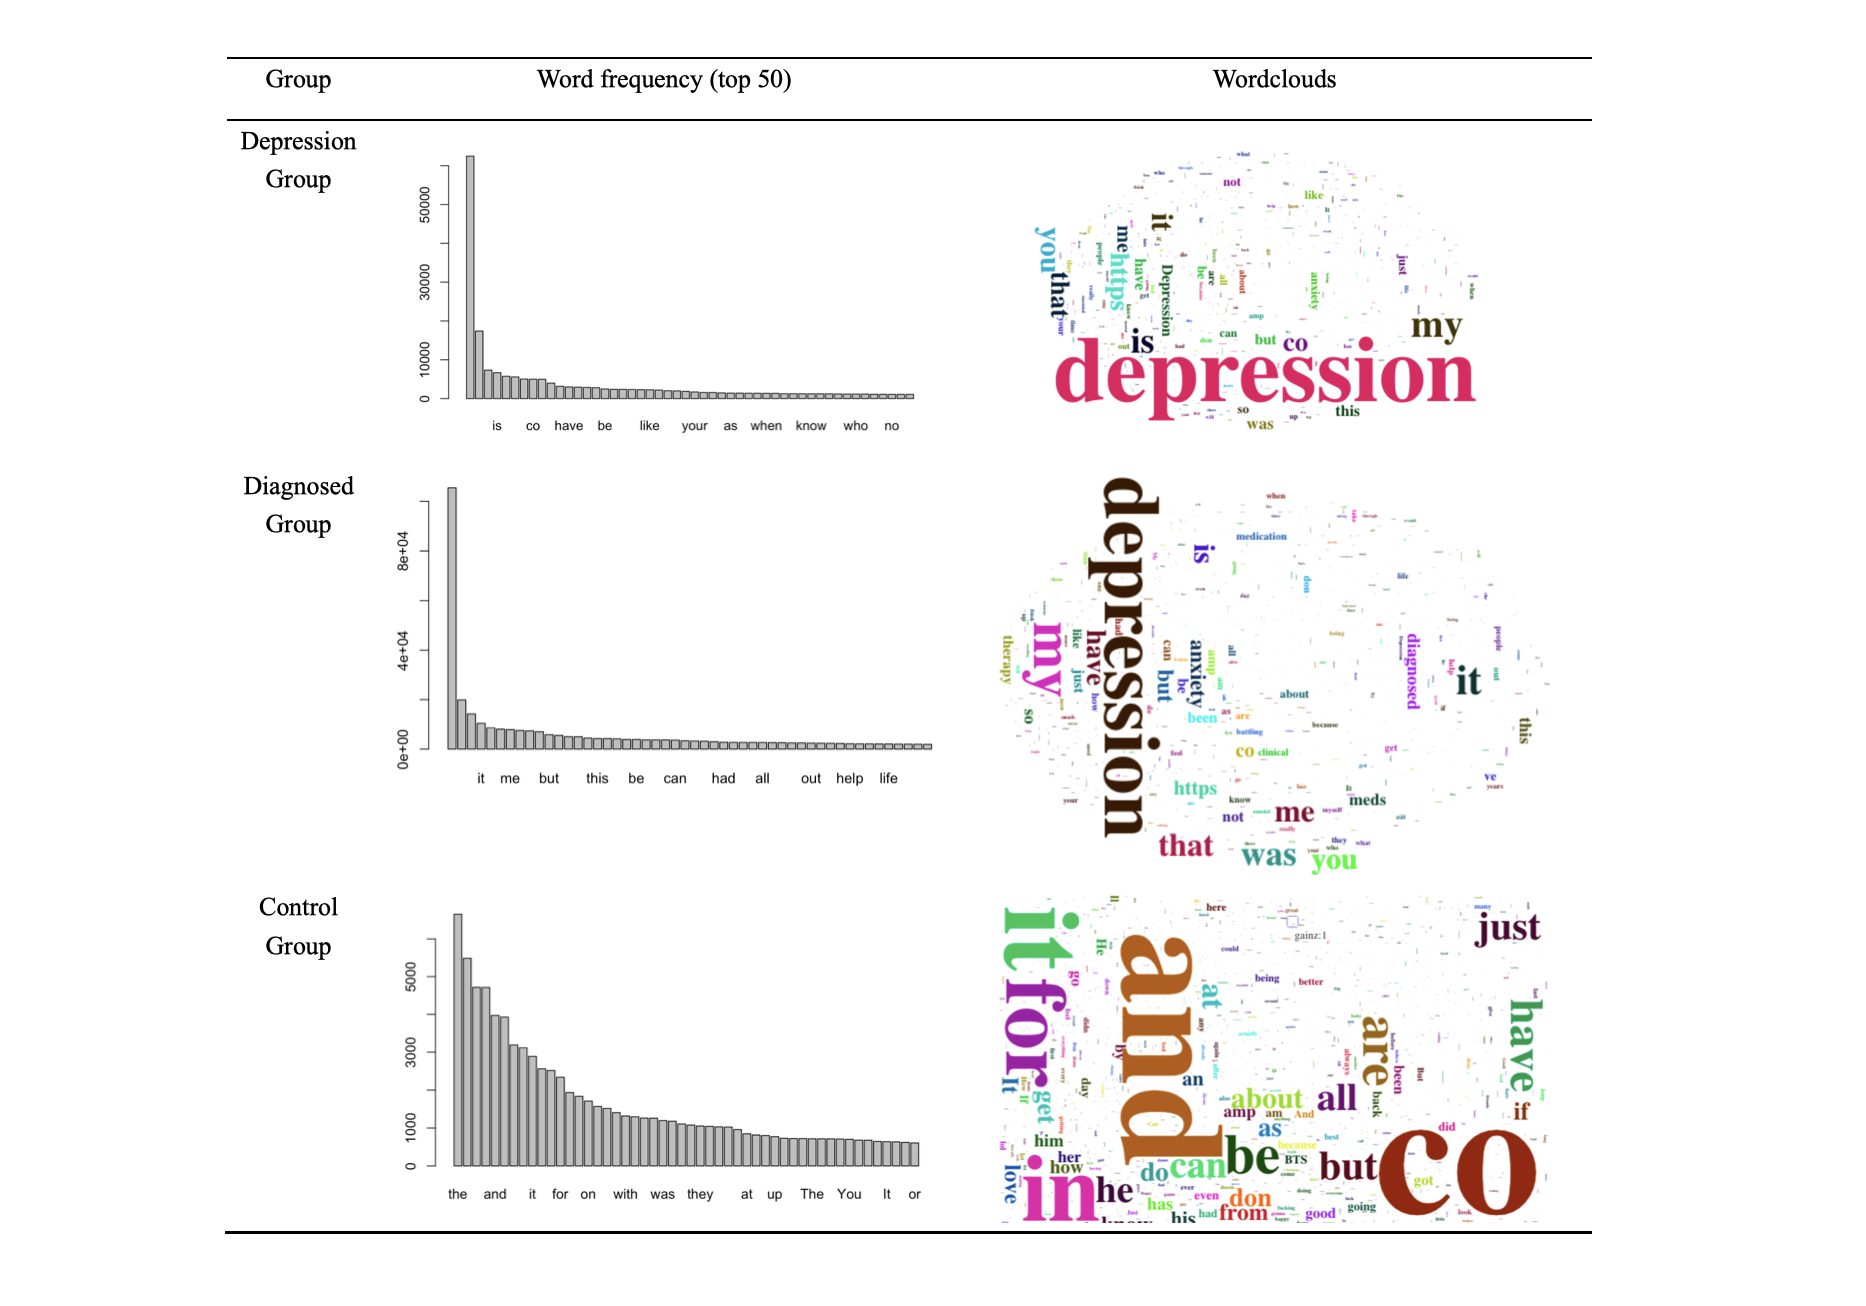
\includegraphics{wordclouds.png}
\caption{Word frequency and wordcloud for each group}
\end{figure}

\begin{Shaded}
\begin{Highlighting}[]
\CommentTok{# Create wordclouds for each group}
\CommentTok{# Group 1}
\NormalTok{dp1_text <-}\StringTok{ }\KeywordTok{as.character}\NormalTok{(dp1}\OperatorTok{$}\NormalTok{text)}
\NormalTok{seg <-}\StringTok{ }\NormalTok{qseg[dp1_text] }\CommentTok{# use seg to cut vocabulary}
\NormalTok{seg <-}\StringTok{ }\NormalTok{seg[}\KeywordTok{nchar}\NormalTok{(seg)}\OperatorTok{>}\DecValTok{1}\NormalTok{] }\CommentTok{# delete words that less than 1 unit}
\NormalTok{seg}
\CommentTok{# Set stopwords}
\NormalTok{all_stops <-}\StringTok{ }\KeywordTok{c}\NormalTok{(}\StringTok{"and"}\NormalTok{,}\StringTok{"of"}\NormalTok{,}\StringTok{"http"}\NormalTok{,}\StringTok{"to"}\NormalTok{,}\StringTok{"for"}\NormalTok{,}\StringTok{"in"}\NormalTok{,}\StringTok{"on"}\NormalTok{,}\StringTok{"the"}\NormalTok{,}\StringTok{"with"}\NormalTok{,}\StringTok{"at"}\NormalTok{,}\StringTok{"or"}\NormalTok{,}\StringTok{"from"}\NormalTok{)}
\NormalTok{seg <-}\StringTok{ }\KeywordTok{removeWords}\NormalTok{(seg, all_stops)}
\NormalTok{seg <-}\StringTok{ }\KeywordTok{table}\NormalTok{(seg)}
\NormalTok{seg_}\DecValTok{50}\NormalTok{ <-}\StringTok{ }\KeywordTok{sort}\NormalTok{(seg, }\DataTypeTok{decreasing =} \OtherTok{TRUE}\NormalTok{)[}\DecValTok{1}\OperatorTok{:}\DecValTok{50}\NormalTok{]}
\CommentTok{# get word frequency (top 50)}
\NormalTok{seg_}\DecValTok{50}
\KeywordTok{barplot}\NormalTok{(seg_}\DecValTok{50}\NormalTok{)}
\KeywordTok{wordcloud2}\NormalTok{(seg,}\DataTypeTok{size =} \DecValTok{2}\NormalTok{, }\DataTypeTok{minRotation =} \OperatorTok{-}\NormalTok{pi}\OperatorTok{/}\DecValTok{2}\NormalTok{, }\DataTypeTok{maxRotation =} \OperatorTok{-}\NormalTok{pi}\OperatorTok{/}\DecValTok{2}\NormalTok{) }\CommentTok{# Create wordcloud}

\CommentTok{# Group 2}
\NormalTok{dp2_text <-}\StringTok{ }\KeywordTok{as.character}\NormalTok{(dp2}\OperatorTok{$}\NormalTok{text)}
\NormalTok{seg <-}\StringTok{ }\NormalTok{qseg[dp2_text] }\CommentTok{# use seg to cut vocabulary}
\NormalTok{seg <-}\StringTok{ }\NormalTok{seg[}\KeywordTok{nchar}\NormalTok{(seg)}\OperatorTok{>}\DecValTok{1}\NormalTok{] }\CommentTok{# delete words that less than 1 unit}
\NormalTok{seg}

\NormalTok{seg <-}\StringTok{ }\KeywordTok{table}\NormalTok{(seg)}
\NormalTok{seg_}\DecValTok{50}\NormalTok{ <-}\StringTok{ }\KeywordTok{sort}\NormalTok{(seg, }\DataTypeTok{decreasing =} \OtherTok{TRUE}\NormalTok{)[}\DecValTok{1}\OperatorTok{:}\DecValTok{50}\NormalTok{]}
\CommentTok{# get word frequency (top 50)}
\NormalTok{seg_}\DecValTok{50}
\KeywordTok{barplot}\NormalTok{(seg_}\DecValTok{50}\NormalTok{)}
\KeywordTok{wordcloud2}\NormalTok{(seg,}\DataTypeTok{size =} \DecValTok{2}\NormalTok{, }\DataTypeTok{minRotation =} \OperatorTok{-}\NormalTok{pi}\OperatorTok{/}\DecValTok{2}\NormalTok{, }\DataTypeTok{maxRotation =} \OperatorTok{-}\NormalTok{pi}\OperatorTok{/}\DecValTok{2}\NormalTok{) }\CommentTok{# Create wordcloud}

\CommentTok{# Group 3}
\NormalTok{dp3_text <-}\StringTok{ }\KeywordTok{as.character}\NormalTok{(dp3}\OperatorTok{$}\NormalTok{text)}
\NormalTok{seg <-}\StringTok{ }\NormalTok{qseg[dp3_text] }\CommentTok{# use seg to cut vocabulary}
\NormalTok{seg <-}\StringTok{ }\NormalTok{seg[}\KeywordTok{nchar}\NormalTok{(seg)}\OperatorTok{>}\DecValTok{1}\NormalTok{] }\CommentTok{# delete words that less than 1 unit}
\NormalTok{seg}
\CommentTok{# Set stopwords}
\NormalTok{all_stops <-}\StringTok{ }\KeywordTok{c}\NormalTok{(}\StringTok{"and"}\NormalTok{,}\StringTok{"of"}\NormalTok{,}\StringTok{"http"}\NormalTok{,}\StringTok{"to"}\NormalTok{,}\StringTok{"for"}\NormalTok{,}\StringTok{"in"}\NormalTok{,}\StringTok{"on"}\NormalTok{,}\StringTok{"the"}\NormalTok{,}\StringTok{"with"}\NormalTok{,}\StringTok{"at"}\NormalTok{,}\StringTok{"or"}\NormalTok{,}\StringTok{"from"}\NormalTok{)}
\NormalTok{seg <-}\StringTok{ }\KeywordTok{removeWords}\NormalTok{(seg, all_stops)}
\NormalTok{seg <-}\StringTok{ }\KeywordTok{table}\NormalTok{(seg)}
\NormalTok{seg_}\DecValTok{50}\NormalTok{ <-}\StringTok{ }\KeywordTok{sort}\NormalTok{(seg, }\DataTypeTok{decreasing =} \OtherTok{TRUE}\NormalTok{)[}\DecValTok{1}\OperatorTok{:}\DecValTok{50}\NormalTok{]}
\CommentTok{# get word frequency (top 50)}
\NormalTok{seg_}\DecValTok{50}
\KeywordTok{barplot}\NormalTok{(seg_}\DecValTok{50}\NormalTok{)}
\KeywordTok{wordcloud2}\NormalTok{(seg,}\DataTypeTok{size =} \DecValTok{2}\NormalTok{, }\DataTypeTok{minRotation =} \OperatorTok{-}\NormalTok{pi}\OperatorTok{/}\DecValTok{2}\NormalTok{, }\DataTypeTok{maxRotation =} \OperatorTok{-}\NormalTok{pi}\OperatorTok{/}\DecValTok{2}\NormalTok{) }\CommentTok{# Create wordcloud}
\end{Highlighting}
\end{Shaded}

\hypertarget{descriptive-analysis}{%
\paragraph{Descriptive analysis}\label{descriptive-analysis}}

To investigate twitter user's online activities, we select five key
variables as user features from tweets data for preliminary descriptive
analysis: source is a categorical variable, and followers count, friends
count, statuses count, and favourites count are continuous variables.
Before conducting descriptive analysis, we identify potential outliers
or influential observations of user features variables through histogram
and boxplot and find that all the four distributions are asymmetric and
highly right-skewed. To reduce the effect brought by extreme values on
data for further analysis, we use median to replace the outliers those
are larger than upper quantile plus 1.5 times upper quantile minus lower
quantile instead of mean, because mean is already influenced by outliers
largely.

\begin{longtable}[]{@{}lllllll@{}}
\toprule
& Min & & & Max & &\tabularnewline
\midrule
\endhead
& G1 & G2 & G3 & G1 & G2 & G3\tabularnewline
followers\_count & 0.00 & 0.00 & 0.00 & 1918.00 & 1919.00 &
1918.00\tabularnewline
friends\_count & 0.00 & 0.00 & 0.00 & 1783.00 & 1783.00 &
1778.00\tabularnewline
statuses\_count & 1.00 & 0.00 & 1.00 & 50010.00 & 50087.00 &
49811.00\tabularnewline
favourites\_count & 0.00 & 0.00 & 0.00 & 54301.00 & 54451.00 &
54425.00\tabularnewline
\bottomrule
\end{longtable}

\begin{longtable}[]{@{}lllllllll@{}}
\caption{Basic statistics about activities of tweeter
user}\tabularnewline
\toprule
Median & & & Mean & & & Std.dev. & &\tabularnewline
\midrule
\endfirsthead
\toprule
Median & & & Mean & & & Std.dev. & &\tabularnewline
\midrule
\endhead
G1 & G2 & G3 & G1 & G2 & G3 & G1 & G2 & G3\tabularnewline
235.00 & 269.00 & 276.00 & 347.53 & 368.95 & 398.17 & 393.03 & 412.66 &
418.62\tabularnewline
306.00 & 339.00 & 351.00 & 391.02 & 411.19 & 451.61 & 358.70 & 374.82 &
372.58\tabularnewline
5645.50 & 5950.00 & 6171.00 & 8944.12 & 9012.25 & 9956.50 & 10948.09 &
10996.06 & 11216.09\tabularnewline
5881.50 & 5238.00 & 6861.00 & 9912.68 & 9365.84 & 12143.14 & 12094.38 &
11861.43 & 12884.63\tabularnewline
\bottomrule
\end{longtable}

\hypertarget{user-features-between-different-groups}{%
\paragraph{User features between different
groups}\label{user-features-between-different-groups}}

\begin{figure}

{\centering \includegraphics[width=0.55\linewidth]{Final-paper-text_files/figure-latex/unnamed-chunk-15-1} 

}

\caption{Feature means: Comparison between groups}\label{fig:unnamed-chunk-15}
\end{figure}

\begin{figure}

{\centering \includegraphics[width=0.55\linewidth]{Final-paper-text_files/figure-latex/unnamed-chunk-16-1} 

}

\caption{Distribution of tweeting sources}\label{fig:unnamed-chunk-16}
\end{figure}

\hypertarget{tweets-time-distribution-between-depression-group-and-diagnosed-group}{%
\paragraph{Tweets time distribution between depression group and
diagnosed
group}\label{tweets-time-distribution-between-depression-group-and-diagnosed-group}}

To probe how the tweets representing depression are distributed during
24 hours over an entire day, we extract the rounded hour of every tweet
issued and calculate the total number of tweets within a certain hour.
Figure 3 shows that the tweets of depression group centralize around
01:00 at late night, with high frequencies from 01:00 to 03:00. This is
probably because depression symptoms tend to worsen during the nights,
also due to the posting patterns that people are generally willing to
use social media after the end of workday. Limited by the tweets of
control group not covering 24 hours over the entire day, we only focus
on the difference between distributions of depression group and
diagnosed group. From Figure 4, we observe that evenings and early
nights show peak, which is same as Figure 3. Line A displays that the
tweets of diagnosed group centralize around 20:00 at night. Line B shows
how the mean of tweets of depression group and diagnosed group changes
over one day. We can still find a diurnal posting pattern with lower
activity through daytime and high activity after 00:00 at late night.
Also, by comparing the ranges of Figure 3 and Figure 4, we observe that
the number of tweets at every hour in diagnosed group (70\% more) has a
larger range than depression group (66\% more).

\begin{verbatim}
## [1] "1997-03-16"
\end{verbatim}

\begin{verbatim}
## [1] "1997-03-16"
\end{verbatim}

\begin{verbatim}
## [1] "1997-03-16"
\end{verbatim}

\begin{verbatim}
## Warning: Ignoring unknown aesthetics: fill
\end{verbatim}

\begin{figure}

{\centering \includegraphics[width=0.55\linewidth]{Final-paper-text_files/figure-latex/unnamed-chunk-18-1} 

}

\caption{Distribution of depression group & diagnosed group tweets in 24 hours}\label{fig:unnamed-chunk-18}
\end{figure}

\begin{figure}

{\centering \includegraphics[width=0.55\linewidth]{Final-paper-text_files/figure-latex/unnamed-chunk-19-1} 

}

\caption{Distribution of depression group tweets in 24 hours}\label{fig:unnamed-chunk-19}
\end{figure}

\hypertarget{analysis}{%
\subsubsection{Analysis}\label{analysis}}

\hypertarget{user-features-means-t-test}{%
\paragraph{User features means
t-test}\label{user-features-means-t-test}}

In order to compare the features of users' Twitter activity, We extend
these findings through observations of the difference in means across
the three groups in terms of various features, including followers
count, friends count, statuses count and favourites count. We conduct
paired sample \emph{t} - test (two-tailed) three times for each feature
to examine whether there is any significant difference between any of
the two groups. The results are summarized in Table xxxxxx.

\begin{longtable}[]{@{}llll@{}}
\caption{Paired t - test for user features}\tabularnewline
\toprule
Group & Difference & \emph{t} -stats & \emph{p} value\tabularnewline
\midrule
\endfirsthead
\toprule
Group & Difference & \emph{t} -stats & \emph{p} value\tabularnewline
\midrule
\endhead
\textbf{Followers count} & & &\tabularnewline
G1 vs.~G2 & -21.4219 & -5.3161 & \textless{} .0001 ***\tabularnewline
G3 vs.~G2 & 29.2185 & 7.0296 & \textless{} .0001 ***\tabularnewline
G1 vs.~G3 & -50.6404 & -12.472 & \textless{} .0001 ***\tabularnewline
\textbf{Friends count} & & &\tabularnewline
G1 vs.~G2 & -20.1694 & -5.498 & \textless{} .0001 ***\tabularnewline
G3 vs.~G2 & 40.4146 & 10.815 & \textless{} .0001 ***\tabularnewline
G1 vs.~G3 & -60.584 & -16.566 & \textless{} .0001 ***\tabularnewline
\textbf{Statuses count} & & &\tabularnewline
G1 vs.~G2 & -68.128 & -0.62092 & 0.5347\tabularnewline
G3 vs.~G2 & 944.252 & 8.5017 & \textless{} .0001 ***\tabularnewline
G1 vs.~G3 & -1012.38 & -9.1346 & \textless{} .0001 ***\tabularnewline
\textbf{Favourites count} & & &\tabularnewline
G1 vs.~G2 & 546.837 & 4.5652 & \textless{} .0001 ***\tabularnewline
G3 vs.~G2 & 2777.293 & 22.427 & \textless{} .0001 ***\tabularnewline
G1 vs.~G3 & -2230.456 & -17.85 & \textless{} .0001 ***\tabularnewline
\bottomrule
\end{longtable}

As can be seen in Table xxxxxx, the independent paired \emph{t} - test
reveals a significant difference between ``Depression Group'' and
``Control Group'' on the number of followers, friends and favourites.
These results suggest that the ``Depression Group'' has significant
fewer followers, fewer friends but more favourites than normal
individuals, all \emph{ts} \textless{} 0.0001. However, there is no
significant difference on the number of statuses. the independent paired
\emph{t} - test reveals a significant difference between ``Diagnosed
Group'' and ``Control Group'' on the number of followers, friends,
statuses and favourites. These results suggest that the ``Diagnosed
Group'' has significant fewer followers, fewer friends , fewer statuses
but also more favourites than normal individuals, all \emph{ts}
\textless{} 0.0001. The results of ``Diagnosed Group'' reflects the
results of ``Depression Group'', indicating that the depressed
individuals might have the same on-line behavior features, which are
different from the control group. Furthermore, we also compared the
``Depression Group'' and the ``Diagnosed Group'', finding that there is
a significant difference between ``Diagnosed Group'' and ``Control
Group'' on the number of followers, friends, statuses and favourites.
``Diagnosed Group'' have more followers, more friends, more statuses and
more favourites than the general ``Depression Group''.

\hypertarget{sentiment-analysis}{%
\paragraph{Sentiment analysis}\label{sentiment-analysis}}

Next we explore the sentiment embedded in tweets of three groups. Before
parsing the information, we extract all the text and clean the data by
deleting non-word characters like punctuations, digits, URLs, and
emojis. Then we take eight different sentiments out of the text through
calling the NRC sentiment dictionary to calculate the presence of eight
emotions and their valence. The ten sentiments are as follows:
``positive'', ``anger'', ``anticipation'', ``disgust'', ``fear'',
``joy'', ``sadness'', ``surprise'', ``trust'', and ``negative''. We use
the mean of each sentiment as score in every group and adjust the
uniform scale of y-axis to (0, 3), in this case comparison between the
scores of each group is more conveniently to be conducted.

\hypertarget{sentiment-score-comparison-within-and-between-groups}{%
\subparagraph{Sentiment score comparison within and between
groups}\label{sentiment-score-comparison-within-and-between-groups}}

Figure 5, 6, and 7 displays the distribution of different sentiments in
each group on the same scale separately. Red columns represent negative
sentiments, green columns represent positive sentiments, and for the
same type of color, the deeper means stronger sentiment. For example,
``joy'' is a stronger positive feeling than ``anticipation''. For Figure
5, we observe that the mean scores of almost every negative sentiment is
higher than positive sentiments overall. Specifically, ``sadness''
(\textgreater{}1.5) and ``negative'' (\textgreater{}2.0) are
significantly higher than the other mean scores, corresponding that user
tweets to express depression on social media. Among the eight exact
different sentiments, the means are not significantly different except
``sadness''. In Figure 6, all the sentiment means are relatively equal
under 0.5 approaching 0, only ``positive'' is larger than 0.5. To some
extent, social media is a platform on which users are more likely to
post in an active or positive emotional state. Figure 7 shows
outstanding differences of means between each sentiment. We find that
``negative'' (\textgreater{}2.5) and ``sadness'' (\textgreater{}2.0) are
much higher than the other sentiments. Among negative sentiments, the
``anger'' and ``fear'' are less expressed in depression tweets, and
``trust'' and ``anticipation'' are more conveyed in depression tweets
compared to ``joy'' and ``surprise''.

\begin{figure}

{\centering \includegraphics[width=0.55\linewidth]{Final-paper-text_files/figure-latex/unnamed-chunk-25-1} 

}

\caption{Distribution of tweets sentiment scores of depression group}\label{fig:unnamed-chunk-25}
\end{figure}

\begin{figure}

{\centering \includegraphics[width=0.55\linewidth]{Final-paper-text_files/figure-latex/unnamed-chunk-26-1} 

}

\caption{Distribution of tweets sentiment scores of control group}\label{fig:unnamed-chunk-26}
\end{figure}

\begin{figure}

{\centering \includegraphics[width=0.55\linewidth]{Final-paper-text_files/figure-latex/unnamed-chunk-27-1} 

}

\caption{Distribution of tweets sentiment scores of diagnosed group}\label{fig:unnamed-chunk-27}
\end{figure}

Between the three groups, control group, pulled under no condition,
shows more flat feelings as a whole compared to depression group and
diagnosed group, and the means of sentiment scores are remarkably lower
than the other groups including depression. Overall, the means in
control group are less than 0.5 and very close to 0, except ``positive''
which is slightly higher than 0.5. However, Figure 5 and 7 show that
there exist obvious differences between means of depression group and
diagnosed group. The emotions expressed in diagnosed group are stronger
than control group, no matter what kind of sentiment it is, particularly
``negative'', ``sadness'', and ``fear'' increase a lot.

\hypertarget{sentimental-analysis-between-different-groups}{%
\subparagraph{Sentimental analysis between different
groups}\label{sentimental-analysis-between-different-groups}}

In order to explore the sentimental difference between different groups,
we conduct independent paired \emph{t} - test on both negative sentiment
and positive sentiment. The results in Table xxxxxxx show that all terms
are statistically significant between either two groups, all \emph{ts}
\textless{} 0.0001. More specifically, in negative sentiment, both
``Depression Group'' and ``Diagnosed Group'' have more negative
sentiment than ``Control Group''. It is easy to understand that people
with depression emotion or self-reported have been diagnosed with
depression, whose Twitter posts will tend to be more negative and
contain more negative words and phrases. Meanwhile, we can see that
``Diagnosed Group'' has significantly more negative sentiment than
``Depression Group'', indicating that there is a difference between
general depressed emotion or feelings and diagnosis of depression. The
later is more serious. It also can be concluded that we could detect
more serious depression through the terms and phrases which we used to
extract ``Diagnosed Group''.

\begin{longtable}[]{@{}llll@{}}
\caption{Paired t - test for sentiment score}\tabularnewline
\toprule
Group & Difference & \emph{t} -stats & \emph{p} value\tabularnewline
\midrule
\endfirsthead
\toprule
Group & Difference & \emph{t} -stats & \emph{p} value\tabularnewline
\midrule
\endhead
\textbf{Negative Sentiment} & & &\tabularnewline
G1 vs.~G2 & 1.68765 & 151.27 & \textless{} .0001 ***\tabularnewline
G3 vs.~G2 & 2.22245 & 189.49 & \textless{} .0001 ***\tabularnewline
G1 vs.~G3 & -0.5348 & -38.251 & \textless{} .0001 ***\tabularnewline
\textbf{Positive Sentiment} & & &\tabularnewline
G1 vs.~G2 & 0.3493 & 31.1 & \textless{} .0001 ***\tabularnewline
G3 vs.~G2 & 0.8627 & 72.615 & \textless{} .0001 ***\tabularnewline
G1 vs.~G3 & -0.5134 & -39.785 & \textless{} .0001 ***\tabularnewline
\bottomrule
\end{longtable}

For positive sentiment, we observe that both ``Depression Group'' and
``Diagnosed Group'' have more positive sentiment than ``Control Group'',
which seems counterintuitive. However, depression is not just a single
symptom, it is usually accompanied by anxiety or even excitement. In
fact, there is a mental health condition called Bipolar Disorder (BP),
which causes extreme mood swings that include emotional highs (mania or
hypomania) and lows (depression). In this circumstance, it might show
bipolar results that the sentiment of depressed or diagnosed depressed
individual appears to be both significant positive and negative. Our
results confirm the objectivity of psychological phenomena in some
aspects.

\hypertarget{user-features-and-sentiment-scores}{%
\subparagraph{User features and sentiment
scores}\label{user-features-and-sentiment-scores}}

To investigate how the user features effect user's sentiment, including
general sentiment, negative sentiment, and positive sentiment, we run
three groups of simple linear regressions, respectively on general
sentiment score, negative sentiment score, and positive sentiment score.
Each group has the same independent variables: followers count, friends
count, statuses count, and favourites count. Dependent variables are
scores of depression group, control group, and diagnosed group.

\begin{longtable}[]{@{}llll@{}}
\caption{Regression test of user features and sentiment
scores}\tabularnewline
\toprule
& depression group & control group & diagnosed group\tabularnewline
\midrule
\endfirsthead
\toprule
& depression group & control group & diagnosed group\tabularnewline
\midrule
\endhead
\textbf{Sentiment score} & & &\tabularnewline
Intercept & -1.109e+00*** & 2.308e-01*** & -1.097e+00***\tabularnewline
Followers\_count & -1.521e-05 & -2.133e-06 & 6.007e-05\tabularnewline
Friends\_count & 3.875e-05 & 1.269e-05 & 6.007e-05***\tabularnewline
Statuses\_count & -2.455e-06* & -2.843e-06*** &
-1.367e-06\tabularnewline
Favourites\_count & -1.562e-07 & -2.843e-06 & 1.361e-06\tabularnewline
\textbf{Negative sentiment score} & & &\tabularnewline
Intercept & 2.131e+00*** & 4.754e-01*** & 2.605e+00***\tabularnewline
Followers\_count & 8.280e-06 & -6.472e-05*** & 4.907e-05\tabularnewline
Friends\_count & 1.012e-04** & 8.478e-06 & 8.653e-05**\tabularnewline
Statuses\_count & 1.012e-04 & 1.260e-06* & -3.077e-07\tabularnewline
Favourites\_count & -1.197e-06 & -2.006e-07 & 2.208e-06*\tabularnewline
\textbf{Positive sentiment score} & & &\tabularnewline
Intercept & 1.022e+00*** & 7.062e-01*** & 1.508e+00***\tabularnewline
Followers\_count & -6.933e-06 & -6.685e-05** &
1.091e-04***\tabularnewline
Friends\_count & 1.400e-04*** & 2.117e-05 & -7.634e-05**\tabularnewline
Statuses\_count & -3.522e-06*** & -1.583e-06* &
-1.675e-06\tabularnewline
Favourites\_count & -1.354e-06 & 4.807e-07 & 3.569e-06***\tabularnewline
\bottomrule
\end{longtable}

Table 2 shows that for general sentiment score, friends count has a
positive effect on general sentiment score of diagnosed people, which
means that the more friends this account has, the higher score it is.
Also, statuses count has positive effects on both depression group and
control group, which means that the more tweets issued, the higher score
they get. For negative sentiment score, we observe that followers count
has a negative effect only on control group, friends count has a
positive effect on diagnosed group, statuses count has a positive effect
on control group, and favourites count has a positive effect on
diagnosed group. As for positive sentiment score, it shows that
followers count have negative effect on control group but positive
effect on diagnosed group, friends count have positive effect on
depression group but negative effect on diagnosed group, statuses count
have both negative effect on depression and control group, and
favourites count has negative effect on diagnosed group.

\hypertarget{discussion}{%
\subsection{Discussion}\label{discussion}}

\hypertarget{conclusions-and-implications}{%
\subsubsection{Conclusions and
implications}\label{conclusions-and-implications}}

\hypertarget{conclusion}{%
\paragraph{Conclusion}\label{conclusion}}

In summary, there are three major findings to emerge from the analysis
of the data from the independent paired \emph{t} - test. ``Depression
Group'' has a significant difference from the control group on the term
of followers count, friends count and favourites count. The individuals
that expressed depressed emotion have less followers and friends. It may
have three explanation. First, they have fewer friends and fewer people
who follow their statuses so that they lack of social support to detect
their depressed emotion while give them emotional support, which could
be the reason that they exhibit an explicit depression on Twitter.
Second, it may because that people would not like to receive negative
emotion and information from social media, then they choose not to
follow or to become friend with depressed individuals. Third, these
accounts could be people's secret social media account that nobody know.
Many people use secret or private account to express their feelings,
especially negative feelings that they do not want others to know. All
the circumstances above could be the reason that ``Depression Group''
has significant fewer followers and friends than the control group.

On the contrary, for ``Diagnosed Group'', the results of independent
paired \emph{t} - test reveals that there is a significant difference
between ``Diagnosed Group'' and ``Control Group'', but it shows that
``Diagnosed Group'' has significant more followers, friends, statuses
and favourites. It seems counterintuitive. We can look at this problem
from two perspectives. First, whether individuals with depression are
likely to attract more friends and followers, and second, whether people
with more friends will show a diagnosis of depression. It is undeniable
that social media like Twitter is a public platform that everyone can
see your posts, so there could be a social desirability that individuals
are likely to show positive emotion and feelings to meet the expectation
of society. It it hard to speak out that `` I am diagnosed with
depression''. However, if someone publicly stated that he/she was
diagnosed with depression, this would give invisible encouragement and
support to others who did not dare to speak. They may choose to follow
this account and gather together, seeking for more resonance. On the
other hand, if an individual has more followers and friends on Twitter,
it means that he or she has more social support, and thus the individual
might have more courage to admit diagnosing depression.

Meanwhile, we find it is interesting that both ``Depression Group'' and
``Diagnosed Group'' tweets have more favourites than control group. It
might because that when people express their depression emotion and
negative thoughts on social media, their friends and followers will
detect and realize that they need social support and would like to use
the ``favourite'' function to show their support and attention to the
individual. People give the depressed tweets ``favourite'' to express
their empathy.

\hypertarget{implications}{%
\paragraph{Implications}\label{implications}}

Unlike previous studies we used depression-related tweets and
diagnosis-related tweets to create our sample study group. We also
compared the tweets with a control group to further validate that the
user behavior from depression individuals and diagnosed depression
individuals will be significantly associated with tweets regarding
symptoms and characteristics of depression. The main contribution of our
study is investigating the relationships between features of Twitter
users and their sentimental performances. We found that people's
activities on social media could be considered as a kind of effective
signal, through which we can detect people's depression. Users with
either general depressed emotion or self-reported diagnosed with
depression do have a significant difference with the normal people. Then
we explore the reasons behind it. It is worth mentioning that the
ability to illustrate and model individual behavior using their social
media data, that can predict depression or even suicided before their
onset. Moreover, the population-scale trends over geography and time may
provide more evidence for clinical traditional diagnoses of depression.
It might be helpful that psychologists diagnose by analyzing patients'
social network data.

\hypertarget{privacy}{%
\paragraph{Privacy}\label{privacy}}

This research revolves around analysis individuals' behavioral features
and leverages information that may be considered sensitive, hence
privacy is important. Meanwhile, in research related to big data on user
behavior, privacy is very noteworthy. We all know that the data we can
obtain from Twitter API is limited, which protects the privacy of users
to some extent. However, we still need to pay attention to ethical
issues when acquiring and analyzing such data. All the data in this
study is public and legal acquisition.

\hypertarget{limitations}{%
\subsubsection{Limitations}\label{limitations}}

Our study has some limitations. While we extract tweets for the control
group, we did not rule out posts that do contain depression-related
terms and phrases. So the control group does not mean that they do not
have depression. Also, there is probability that people do have
depression but they have not tweeted about it. We can not detect and
exclude them from our dataset and more rigorous measures should be
taken. Moreover, due to the ability of API to collect data, the tweets
in control group do not cover all the time periods of a day. It might
cause errors in our analysis process. We did not look over every tweets
to identify whether they truly represent the individual's mental state,
for more reliable results, we need to do that. Since mental health is a
general concept and even depression could be accompanied by other mental
illness. Future studies need to address other mental illnesses that may
co-exist with depression that can also impact symptomatic tweets.

\hypertarget{references}{%
\subsection*{References}\label{references}}
\addcontentsline{toc}{subsection}{References}

\hypertarget{refs}{}
\leavevmode\hypertarget{ref-CDC2008}{}%
Centers for Disease Control and Prevention (CDC). 2012. ``Behavioral
Risk Factor Surveillance System Survey Data.'' \emph{U.S. Department of
Health and Human Services, Centers for Disease Control and Prevention},
1348--53.

\leavevmode\hypertarget{ref-MChoudhury2013}{}%
Choudhury, Munmun De., Scott Counts, and Eric Horvitz. 2013. ``Social
Media as a Measurement Tool of Depression in Populations.''
\emph{Proceedings of the 5th Annual ACM Web Science Conference}. ACM,
47--56.

\leavevmode\hypertarget{ref-Choudhury2013}{}%
Choudhury, Munmun De., Michael Gamon, Scott Counts, and Eric Horvitz.
2013. ``Predicting Depression via Social Media.'' \emph{Seventh
International AAAI Conference on Weblogs and Social Media}. IEEE,
2906--13.

\leavevmode\hypertarget{ref-Luoma2002}{}%
Luoma, Jason B., Catherine E. Martin, and Jane L. Pearson. 2002.
``Contact with Mental Health and Primary Care Providers Before Suicide:A
Review of the Evidence.'' \emph{American Journal of Psychiatry} 159 (6):
909--16.

\leavevmode\hypertarget{ref-Park2012}{}%
Park, Minsu, Chiyoung Cha, and Meeyoung Cha. 2012. ``Depressive Moods of
Users Portrayed in Twitter.'' \emph{Proceedings of the ACM SIGKDD
Workshop on Healthcare Informatics} 2012: 1--8.

\leavevmode\hypertarget{ref-Resnik2013}{}%
Resnik, Philip, Anderson Garron, and Rebecca Resnik. 2013. ``Using Topic
Modeling to Improve Prediction of Neuroticism and Depression in College
Students.'' \emph{Proceedings of the 2013 Conference on Empirical
Methods in Natural Language Processing}, 1348--53.

\leavevmode\hypertarget{ref-Rosenquist2011}{}%
Rosenquist, J.N., J.H. Fowler, and N.A. Christakis. 2002. ``Contact with
Mental Health and Primary Care Providers Before Suicide:A Review of the
Evidence.'' \emph{Molecular Psychiatry} 16 (3): 273--81.

\leavevmode\hypertarget{ref-Smith2013}{}%
Smith, Katie M., Perry F. Renshaw, and John Bilello. 2013. ``Quantifying
Mental Health Signals in Twitter.'' \emph{Comprehensive Psychiatry} 54
(1): 1--6.

\leavevmode\hypertarget{ref-Tsugawa2015}{}%
Tsugawa, Sho, Yusuke Kikuchi, Fumio Kishino, Kosuke Nakajima, Yuichi
Itoh, and Hiroyuki Ohsaki. 2015. ``Recognizing Depression from Twitter
Activity.'' \emph{Proceedings of the 33rd Annual ACM Conference on Human
Factors in Computing Systems}. ACM, 3187--96.


\end{document}
